\documentclass[12pt]{report}
\setcounter{tocdepth}{4}
\setcounter{secnumdepth}{4}

% to insert a title at the beginning of each page
% http://ctan.mirror.garr.it/mirrors/CTAN/info/italian/fancyhdr/itfancyhdr.pdf
\usepackage{fancyhdr}
\pagestyle{fancy}
\lhead{}
\rhead{}
\chead{micro Hayekian Market}


\usepackage{geometry}                % See geometry.pdf to learn the layout options. There are lots.
\geometry{a4paper}                   % ... or a4paper or a5paper or ... letterpaper
%\geometry{landscape}                % Activate for for rotated page geometry
%\usepackage[parfill]{parskip}    % Activate to begin paragraphs with an empty line rather than an indent
\usepackage{graphicx}
\usepackage{amssymb}
\usepackage{epstopdf}
\usepackage[hyphens]{url}         %[hyphens] to break long urls
\usepackage{t1enc} %per uso di caratteri come << >>
%\DeclareGraphicsRule{.tif}{png}{.png}{`convert #1 `dirname #1`/`basename #1 .tif`.png}

\usepackage{verbatim} %to use \begin{comment} \end{comment}
\usepackage{float} % to use H as rigid placement of a figure after the text, allowing empty spaces

\usepackage{fancyvrb}  % http://texdoc.net/texmf-dist/doc/latex/fancyvrb/fancyvrb.pdf

\usepackage{enumitem} % to avoid bold in description item and to maintain bullets

\usepackage[toc,page]{appendix}

\usepackage{keystroke} % to use \Return

\newcommand{\repeatfootnote}[1]{\textsuperscript{\ref{#1}}} %to repeat a reference


% to have clickable links and references
\usepackage[dvipsnames]{xcolor} % colors at https://en.wikibooks.org/wiki/LaTeX/Colors
\usepackage{xcolor}   %Maybe necessary if you want to color links (better use xcolor than color, more at http://repositorios.cpai.unb.br/ctan/macros/latex/contrib/xcolor/xcolor.pdf)
\usepackage{hyperref}
\hypersetup{
    colorlinks=true, %set true if you want colored links
    linktoc=all,     %set to all if you want both sections and subsections linked
    linkcolor=Brown,  %choose some color if you want links to stan
    urlcolor=cyan,
    citecolor=purple}
    
\usepackage{chngcntr}                      % to avoid restart note numbers 
\counterwithout{footnote}{chapter}    % changing chapter

\usepackage{makeidx}   % creating index (in Italian Indice analitico)

\usepackage{empheq}

\usepackage{tablefootnote} % to use \footnote as \tablefootnote

\newcommand{\ts}{\textsuperscript} %to write briefly th etc. as a superscript

\usepackage{color}
\usepackage{listings}


\makeindex



\title{micro Hayekian Market}
%\subtitle{a}
\author{Matteo Morini\footnote{University of Torino, Italia} and Pietro Terna\footnote{University of Torino, Italia}}

%\date{} %attivare vuoto per eliminare la data oppure attivarne una dichiarata

%\usepackage[square]{natbib}
\usepackage[round]{natbib}

\setlength\fboxsep{0pt}

\renewcommand{\thesection}{\arabic{section}} % to avoid leading zeros in numbering the sections, having eliminate
                                                                           % the Chapter 1 supertitle (see below: to eliminate the Chapter 1 supertitle)

\begin{document}
\maketitle
\thispagestyle{fancy}

\tableofcontents
\thispagestyle{fancy}

\listoffigures
\thispagestyle{fancy}


%%%%%%%%%%%%%%%%%%%%%%%%%%%%%%%%%%%%%%%%%%%%
%%%%%%%%%%%%%%%%%%%%%%%%%%%%%%%%%%%%%%%%%%%%
\chapter*{Introduction to a micro Hayekian Market}
%The * above is to eliminate the Chapter 1 supertitle
\label{micro Hayekian Market}\index{introduction to a micro Hayekian Market}
\thispagestyle{fancy}
\addcontentsline{toc}{chapter}{\protect\numberline{}Introduction to a micro Hayekian Market}%


The purpose of the note is that of introducing a very simple agent-based model of a market, with emergent (quite interesting)  price dynamics.

 A counter example is also introduced, showing how with tiny modification we generate implausible price dynamics.

The code uses the IPython\footnote{\url{https://ipython.org}.} language (interaction with Python\footnote{\url{https://www.python.org}.}) and can be dowloaded from \url{https://github.com/terna/microHayekianMarket} using the \emph{Clone or download} button; it is also possible to run it directly on line at \\\url{https://mybinder.org/v2/gh/terna/microHayekianMarket/master?filepath=microHayekianMarket.ipynb}.

A suggested reading about Hayek is a quite recent paper of \citeauthor{10.1257/jep.31.3.215} (\citeyear{10.1257/jep.31.3.215}).


%%%%%%%%%%%%%%%%%%%%%%%%%%%%%%%%%%%%%%%%%%%%
\section{The technical setup}\label{The technical setup}\index{technical setup}

The IPython (or Python 3.x) code requires the following starting setup:

\begin{lstlisting}[language=Python, caption=Setup of the program, basicstyle=\ttfamily\footnotesize]
%pylab inline
import statistics as s
import numpy as np
import pylab as plt
from IPython.display import clear_output
import time
\end{lstlisting}

\verb|%pylab inline| 
is a \emph{magic} command of Jupyter.\footnote{\url{http://jupyter.org}.}

%%%%%%%%%%%%%%%%%%%%%%%%%%%%%%%%%%%%%%%%%%%%
\section{The structure of the model and the \emph{warming up} phase}\label{The structure of the model}\index{structure}

Our agents are simply prices, to be interpreted as reservation prices.\footnote{The $max$ price a buyer could pay and the $min$ one a seller could accept.}

We have two price vectors: $pL^b$ with item $pL^b_i$ for the buyers, and $pL^s$ with item $pL^s_j$ for the sellers. The $i^{th}$ or the $j^{th}$ elements of the vectors are prices, but  we can use them also as agents.

Both in the hayekian perspective (Section \ref{The hayekian version}) and in the unstructured one (Section \ref{The unstructured version}) we have to pre-run the \emph{warning up} action.

In this phase, we define:

\begin{itemize}
\item $nCycles$ - number of simulation cycles;
\item $nBuyers$  - number of the buyers;
\item $nSellers$ - number of the sellers;
\item $d_0$ - the lower bound of the random uniform numbers, both for the buyers and the sellers, in the warming up phase; 

in the running phase, the lower bound is $0$;
\item $d_1$ - the upper bound of the random uniform numbers for the buyers;
\item $d_2$ - the upper bound of the random uniform numbers for the sellers;
\item the initial buyer $i$ reservation price, different for each buyer: $p_{b,i}=\frac{1} {1 + u_i}$ with $u_i\sim\mathcal{U}(d_0,d_1)$;
\item the initial seller $j$ reservation price, different for each seller: $p_{s,j}=1 + u_j$ with $u_j\sim\mathcal{U}(d_0,d_2)$.
\end{itemize}

With  $d_0=0.1$, $d_1=0.2$, $d_2=0.2$, sorting in decreasing order the vector  $pL^b$ and in increasing order the vector  $pL^s$ we obtain two not overlapping price sequences that we can interpret as a demand curve and an offer one (Fig. \ref{output_2_1.png}).

\begin{figure}[htbp]
\begin{center}
\fbox{\centering 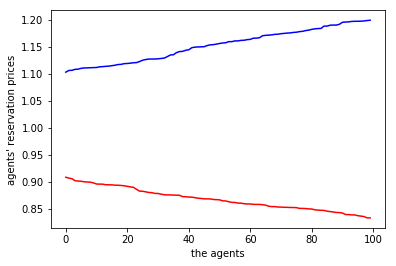
\includegraphics[width=0.6\textwidth]{output_2_1.png}}
\caption{An example of initial not overlapping demand curve and offer curve}
\label{output_2_1.png}
\end{center}
\end{figure}

This is the \emph{warming up}, or starting situation, of the model. To generate new examples related to Section \ref{The hayekian version} and to Section \ref{The unstructured version}, it is necessary to repeat this phase.

The IPython (or Python 3.x) code is:

\begin{lstlisting}[language=Python, caption=Warming up of the model, basicstyle=\ttfamily\footnotesize]
# warming up

# run it before executing both - the hayekian perspective or
#                              - the unstructured case

d0=0.1
d1=0.2
d2=0.2

nCycles=10000
nBuyers= 100
nSellers=100

buyerPriceList=[]
sellerPriceList=[]

for i in range(nBuyers):
    buyerPriceList.append(1/(1+np.random.uniform(d0,d1)))
for j in range(nSellers):
    sellerPriceList.append(1+np.random.uniform(d0,d2))
    
plt.plot(np.sort(buyerPriceList)[::-1],"r");
plt.plot(np.sort(sellerPriceList),"b");
xlabel("the agents");
ylabel("agents' reservation prices");
\end{lstlisting}

%%%%%%%%%%%%%%%%%%%%%%%%%%%%%%%%%%%%%%%%%%%%
\section{The hayekian version}\label{The hayekian version}\index{hayekian version}
 
The buyers and the sellers meet randomly. Buyer $i$ and seller $j$ exchange if  $pL^b_i \geq pL^s_j$; the deal is recorded at the price of the seller $pL^s_j$.\footnote{In the $mall$, sell prices are public.}

In this version, representing the key point in this note, the running prices are changing being multiplied in each cycle by following the correction coefficients:

\begin{itemize}
\item for the buyer: (i) $c_b=\frac{1} {1 + u_b}$ if the deal succeeds (trying the pay less next time) or (ii) $c_b=1 + u_b$ if the deal fails (preparing to pay more next time); in (i) and (ii) we have $u_b\sim\mathcal{U}(0,d_1)$

\item for the seller: (iii) $c_s=1 + u_s$ if the deal succeeds (preparing to obtain a higher revenue next time) or (iv) $c_s=\frac{1} {1 + u_s}$  if the deal fails (preparing to obtain a lower revenue next time); in (iii) and (iv) we have $u_s\sim\mathcal{U}(0,d_2)$.
\end{itemize}

With $d_1=0.2$, $d_2=0.2$ and $nCycles$ set to $10,000$ we obtain sequences of mean prices (mean in each cycle) quite realistic, with a very low variance within each cycle (see Fig. \ref{output_3_1.png} and \ref{output_3_2.png}).

\begin{figure}[htbp]
\begin{center}
\fbox{\centering 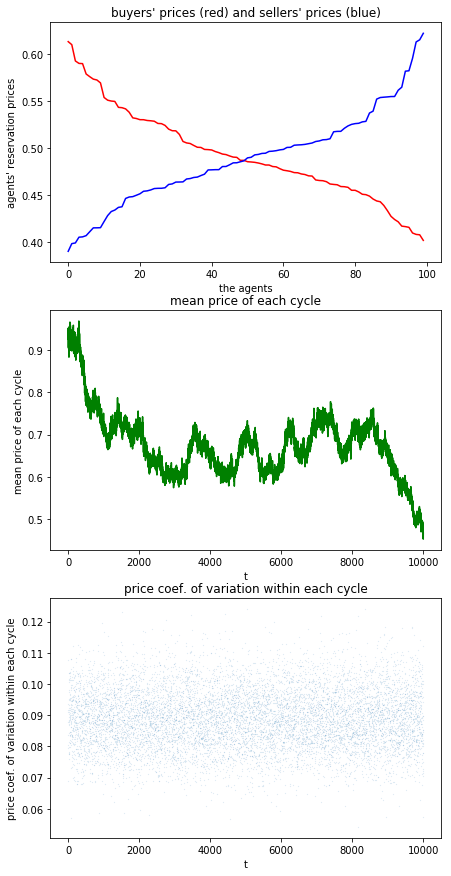
\includegraphics[width=0.6\textwidth]{output_3_1.png}}
\caption{Hayekian case: (i) an example of final demand and offer curves, (ii) the history of mean prices, (iii) their coeffcients of variation within each cycle}
\label{output_3_1.png}
\end{center}
\end{figure}

The \emph{coefficient of variation} at time $t$ is calculated as: $$\frac{standard~deviation_t}{mean_t}$$.

\begin{figure}[htbp]
\begin{center}
\fbox{\centering 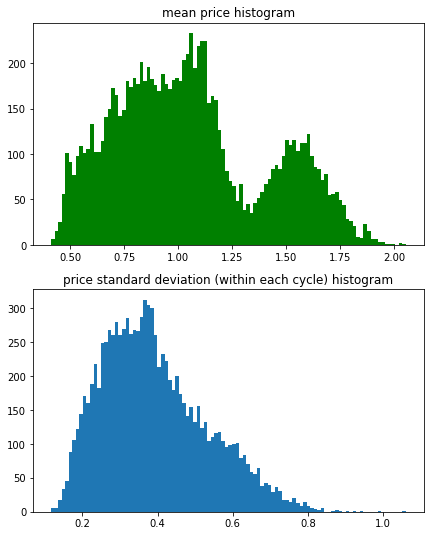
\includegraphics[width=0.6\textwidth]{output_3_2.png}}
\caption{Hayekian case: (i) the distribution of mean prices in each cycle and (ii) that of their standard deviations within each cycle}
\label{output_3_2.png}
\end{center}
\end{figure}

\begin{center}
\fbox{\parbox[c][3.5cm][c]{13cm}{
A comment: we have a plausible series of mean prices, with a complicated behavior, and with a high stability of the dispersion of the values within each cycle.

The right side of the buyer and seller curves shows another plausible situation: that of the presence of agents not exchanging. {\color{red}A note for Matteo and Pietro: this is a very important effect for the \emph{Oligopoly} model.}}}
\end{center}

\bigskip

Have a look to the Appendix \ref{Two cases of not balancing numbers of buyers and sellers} for the cases of not balancing number of buyers and sellers.

The IPython (or Python 3.x) code is:

\begin{lstlisting}[language=Python, caption=The model in the hayekian perspective, basicstyle=\ttfamily\footnotesize]
# hayekian perspective
meanPrice_ts=[]
meanPriceStDev_ts=[]
meanPriceVar_ts=[]

for t in range(1,nCycles+1):    
    dealPrices=[]
    agNum=max(nBuyers,nSellers)
    for n in range(agNum):
        i = np.random.randint(0,nBuyers)
        j = np.random.randint(0,nSellers)
        #print ('%2d %2d %.3f %.3f %.3f'% \
        #      (i,j,buyerPriceList[i]-sellerPriceList[j],\
        #       buyerPriceList[i],sellerPriceList[j]))
        
        if buyerPriceList[i]>=sellerPriceList[j]:
            dealPrices.append(sellerPriceList[j])
            buyerPriceList[i] *=1/(1+np.random.uniform(d1))
            sellerPriceList[j]*=1+np.random.uniform(d2)
        else:
            buyerPriceList[i] *=1+np.random.uniform(d1)
            sellerPriceList[j]*=1/(1+np.random.uniform(d2))

        #print ('%2d %2d %.3f %.3f %.3f \n'% \
        #      (i,j,buyerPriceList[i]-sellerPriceList[j],\
        #       buyerPriceList[i],sellerPriceList[j]))
           
    if len(dealPrices) > 2:
        meanPrice_ts.append(s.mean(dealPrices))
        meanPriceVar_ts.append(s.variance(dealPrices))
        meanPriceStDev_ts.append(s.stdev(dealPrices))
    else:
        meanPrice_ts.append(np.nan)
        meanPriceStDev_ts.append(np.nan)

    if t % 1000==0:
        clear_output()
        print('time', t, 'and n. of exchanges in the last cycle', \
              len(dealPrices))
        print(\
        'mean and var of exchange prices in the last cycle: %.3f, %.3f' %\
              (meanPrice_ts[-1],meanPriceVar_ts[-1]))

        plt.figure(1,figsize=(7,15),clear=True)

        plt.subplot(311)
        plt.plot(np.sort(buyerPriceList)[::-1],"r")
        plt.plot(np.sort(sellerPriceList),"b")
        plt.title(\
            "buyers' prices (red) and sellers' prices (blue)")
        xlabel("the agents")
        ylabel("agents' reservation prices")

        plt.subplot(312)
        plt.title("mean price of each cycle")
        xlabel("t")
        ylabel("mean price of each cycle")
        plt.plot(meanPrice_ts,"g")
        
        plt.subplot(313)
        plt.title("price coef. of variation within each cycle")
        coefOfVariation=[]
        for m in range(len(meanPriceStDev_ts)):
            coefOfVariation.append(meanPriceStDev_ts[m]/
                                   meanPrice_ts[m])
        plt.plot(coefOfVariation,".",markersize=0.1)
        xlabel("t")
        ylabel("price coef. of variation within each cycle")
        show()
        #time.sleep(0.1)

plt.figure(2,figsize=(7,9))
plt.subplot(211)
plt.title("mean price histogram")
plt.hist(meanPrice_ts,100,color="g");
plt.subplot(212)
plt.title("price standard deviation (within each cycle) histogram")
plt.hist(meanPriceStDev_ts,100);
\end{lstlisting}


%%%%%%%%%%%%%%%%%%%%%%%%%%%%%%%%%%%%%%%%%%%%
\section{The unstructured version}\label{The unstructured version}\index{unstructured version}

The buyers and the sellers meet randomly as in Section \ref{The hayekian version}. Buyer $i$ and seller $j$ exchange in any case; the deal is recorded at the mean of the price of the seller $pL^s_j$ and of the price $pL^b_i$ of the buyer.

In this version the running prices are changing being multiplied in each cycle by following the correction coefficients:

\begin{itemize}

\item with the same probability for the buyer: (i) $c_b=\frac{1} {1 + u_b}$ or (ii) $c_b=1 + u_b$); in (i) and (ii) we have $u_b\sim\mathcal{U}(0,d_1)$

\item  with the same probability for the seller: (iii) $c_s=1 + u_s$ or (iv) $c_s=\frac{1} {1 + u_s}$; in (iii) and (iv) we have $u_s\sim\mathcal{U}(0,d_2)$.
\end{itemize}

With $d_1=0.2$, $d_2=0.2$ and $nCycles$ set to $10,000$ we obtain exploding sequences of mean prices (mean in each cycle), and exploding standard deviation within each cycle (see Fig. \ref{output_4_1.png} and \ref{output_4_2.png}).

\begin{figure}[htbp]
\begin{center}
\fbox{\centering 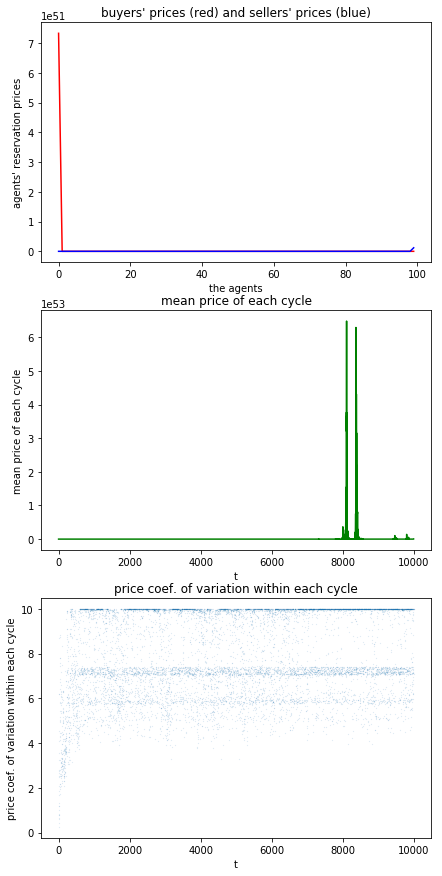
\includegraphics[width=0.6\textwidth]{output_4_1.png}}
\caption{Unstructured case: (i) an example of final demand and offer curves, (ii) the history of mean prices, (iii) their coeffcients of variation within each cycle}
\label{output_4_1.png}
\end{center}
\end{figure}

The \emph{coefficient of variation} at time $t$ is calculated as: $$\frac{standard~deviation_t}{mean_t}$$.

\begin{figure}[htbp]
\begin{center}
\fbox{\centering 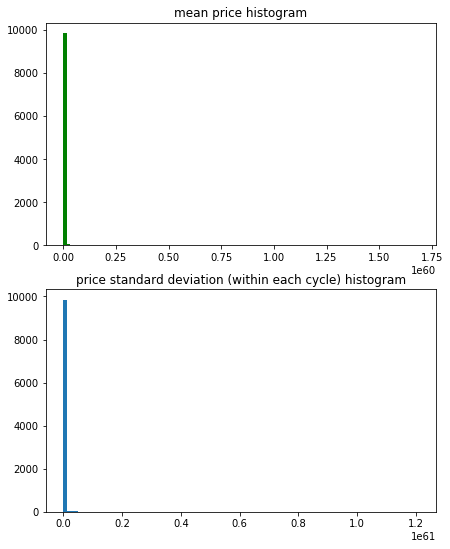
\includegraphics[width=0.6\textwidth]{output_4_2.png}}
\caption{Unstructured case: (i) the distribution of mean prices in each cycle and (ii) that of their standard deviations within each cycle}
\label{output_4_2.png}
\end{center}
\end{figure}

\begin{center}
\fbox{\parbox[c][2.6cm][c]{13cm}{
A comment: this counter-example shows that, missing the \emph{intelligence} in the correction of the prices (implicitly propagating among all the agents), a system of pure random price settings is absolutely far from being plausible.}}
\end{center}

\bigskip

The IPython (or Python 3.x) code is:

\begin{lstlisting}[language=Python, caption=The unstructured version, basicstyle=\ttfamily\footnotesize]
# unstructured case (remember the warming up step)
meanPrice_ts=[]
meanPriceStDev_ts=[]
meanPriceVar_ts=[]

for t in range(1,nCycles+1):    
    dealPrices=[]
    agNum=max(nBuyers,nSellers)
    for n in range(agNum):
        i = np.random.randint(0,nBuyers)
        j = np.random.randint(0,nSellers)
        #print ('%2d %2d %.3f %.3f %.3f'% \
        #      (i,j,buyerPriceList[i]-sellerPriceList[j],\
        #       buyerPriceList[i],sellerPriceList[j]))
        
        dealPrices.append((sellerPriceList[j]+buyerPriceList[i]/0.5))
        
        if np.random.uniform(0,1)>=0.5:    
            buyerPriceList[i] *=1/(1+np.random.uniform(0,d1))
            sellerPriceList[j]*=1+np.random.uniform(0,d2)
        else:
            buyerPriceList[i] *=1+np.random.uniform(0,d1)
            sellerPriceList[j]*=1/(1+np.random.uniform(0,d2))

        #print ('%2d %2d %.3f %.3f %.3f \n'% \
        #      (i,j,buyerPriceList[i]-sellerPriceList[j],\
        #       buyerPriceList[i],sellerPriceList[j]))
           
    if len(dealPrices) > 2:
        meanPrice_ts.append(s.mean(dealPrices))
        meanPriceVar_ts.append(s.variance(dealPrices))
        meanPriceStDev_ts.append(s.stdev(dealPrices))
    else:
        meanPrice_ts.append(np.nan)
        meanPriceStDev_ts.append(np.nan)

    if t % 1000==0:
        clear_output()
        print('time', t, 'and n. of exchanges in the last cycle', \
              len(dealPrices))
        print(\
        'mean and var of exchange prices in the last cycle: %.3f, %.3f' %\
              (meanPrice_ts[-1],meanPriceVar_ts[-1]))

        plt.figure(1,figsize=(7,15),clear=True)

        plt.subplot(311)
        plt.plot(np.sort(buyerPriceList)[::-1],"r")
        plt.plot(np.sort(sellerPriceList),"b")
        plt.title(\
            "buyers' prices (red) and sellers' prices (blue)")
        xlabel("the agents")
        ylabel("agents' reservation prices")

        plt.subplot(312)
        plt.title("mean price of each cycle")
        xlabel("t")
        ylabel("mean price of each cycle")
        plt.plot(meanPrice_ts,"g")
        
        plt.subplot(313)
        plt.title("price coef. of variation within each cycle")
        coefOfVariation=[]
        for m in range(len(meanPriceStDev_ts)):
            coefOfVariation.append(meanPriceStDev_ts[m]/
                                   meanPrice_ts[m])
        plt.plot(coefOfVariation,".",markersize=0.1)
        xlabel("t")
        ylabel("price coef. of variation within each cycle")
        show()
        #time.sleep(0.1)

plt.figure(2,figsize=(7,9))
plt.subplot(211)
plt.title("mean price histogram")
plt.hist(meanPrice_ts,100,color="g");
plt.subplot(212)
plt.title("price standard deviation (within each cycle) histogram")
plt.hist(meanPriceStDev_ts,100);
\end{lstlisting}




\begin{appendices}
%%%%%%%%%%%%%%%%%%%%%%%%%%%%%%%%%%%%%%%%%%%%
%%%%%%%%%%%%%%%%%%%%%%%%%%%%%%%%%%%%%%%%%%%%
\section{Two cases of not balancing numbers of buyers and sellers}\index{not balancing number of buyers and sellers}\label{Two cases of not balancing numbers of buyers and sellers}
\thispagestyle{fancy}

%%%%%%%%%%%%%%%%%%%%%%%%%%%%%%%%%%%%%%%%%%%%
\subsection{Case $nBuyers \gg nSellers$}
If $nBuyers \gg nSellers$ (e.g., $nBuyers=100$ and $nSellers=50$, as in Fig. \ref{output_2_1a.png}), we observe in that Figs. \ref{output_3_1a.png} and \ref{output_3_2a.png} the prices are higher than in Figs. \ref{output_3_1.png} and \ref{output_3_2.png}.

The result is highly consistent with the numbers of the agents in the two sides of the market.

\begin{figure}[htbp]
\begin{center}
\fbox{\centering 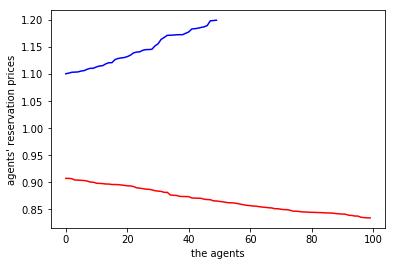
\includegraphics[width=0.6\textwidth]{output_2_1a.png}}
\caption{An example of initial not overlapping demand curve and offer curve, case $nBuyers \gg nSellers$}
\label{output_2_1a.png}
\end{center}
\end{figure}

\begin{figure}[htbp]
\begin{center}
\fbox{\centering 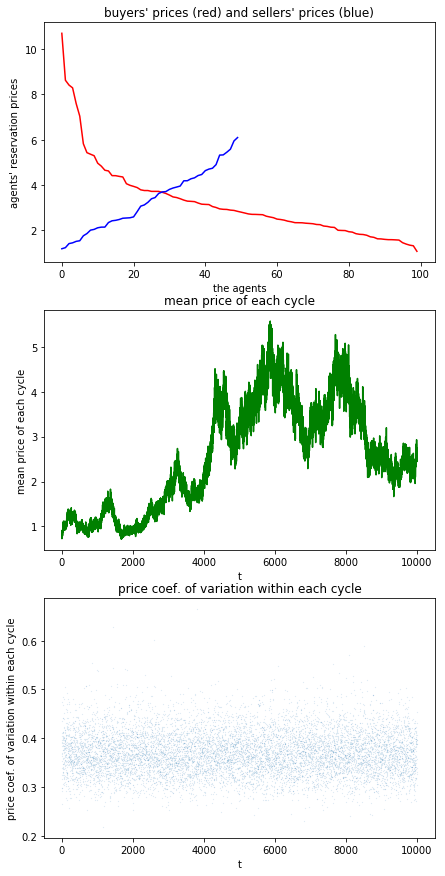
\includegraphics[width=0.6\textwidth]{output_3_1a.png}}
\caption{Hayekian case, with $nBuyers \gg nSellers$: (i) an example of final demand and offer curves, (ii) the history of mean prices, (iii) their coeffcients of variation within each cycle}
\label{output_3_1a.png}
\end{center}
\end{figure}

\begin{figure}[htbp]
\begin{center}
\fbox{\centering 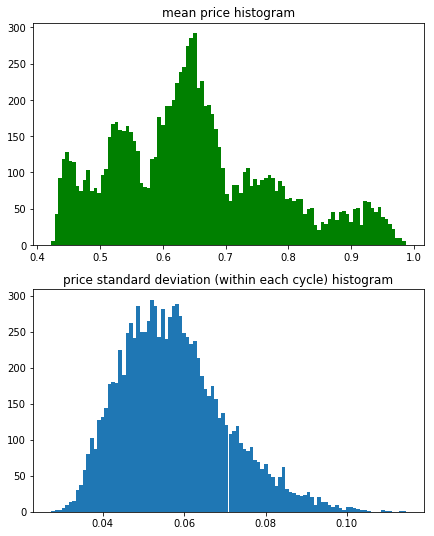
\includegraphics[width=0.6\textwidth]{output_3_2a.png}}
\caption{Hayekian case, with $nBuyers \gg nSellers$: (i) the distribution of mean prices in each cycle and (ii) that of their standard deviations within each cycle}
\label{output_3_2a.png}
\end{center}
\end{figure}

%%%%%%%%%%%%%%%%%%%%%%%%%%%%%%%%%%%%%%%%%%%%
\subsection{Case $nBuyers \ll nSellers$}
If $nBuyers \ll nSellers$ (e.g., $nBuyers=50$ and $nSellers=100$, as in Fig. \ref{output_2_1b.png}), we observe in that Figs. \ref{output_3_1b.png} and \ref{output_3_2b.png} the prices are lower than in Figs. \ref{output_3_1.png} and \ref{output_3_2.png}.

The result is highly consistent with the numbers of the agents in the two sides of the market.


\begin{figure}[htbp]
\begin{center}
\fbox{\centering 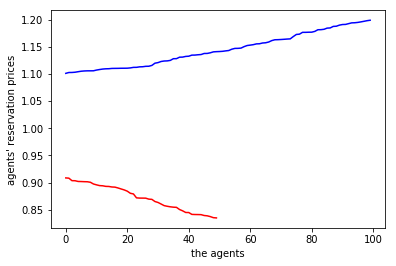
\includegraphics[width=0.6\textwidth]{output_2_1b.png}}
\caption{An example of initial not overlapping demand curve and offer curve, case $nBuyers \ll nSellers$}
\label{output_2_1b.png}
\end{center}
\end{figure}

\begin{figure}[htbp]
\begin{center}
\fbox{\centering 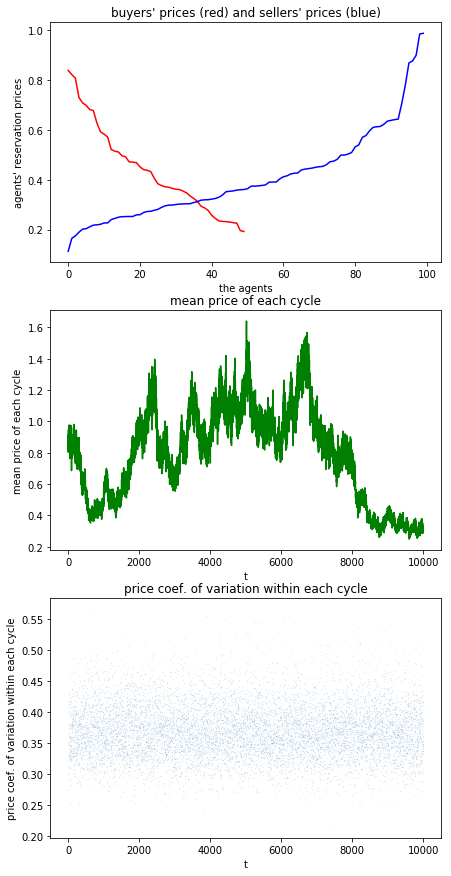
\includegraphics[width=0.6\textwidth]{output_3_1b.png}}
\caption{Hayekian case, with $nBuyers \ll nSellers$: (i) an example of final demand and offer curves, (ii) the history of mean prices, (iii) their coeffcients of variation within each cycle}
\label{output_3_1b.png}
\end{center}
\end{figure}

\begin{figure}[htbp]
\begin{center}
\fbox{\centering 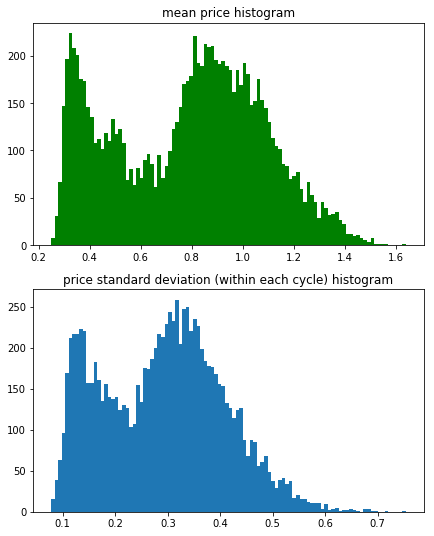
\includegraphics[width=0.6\textwidth]{output_3_2b.png}}
\caption{Hayekian case, with $nBuyers \ll nSellers$: (i) the distribution of mean prices in each cycle and (ii) that of their standard deviations within each cycle}
\label{output_3_2b.png}
\end{center}
\end{figure}



\end{appendices}

\clearpage
\addcontentsline{toc}{chapter}{Bibliography}
\bibliography{./bibliografiaGenerale}
\bibliographystyle{plainnatmm}


\clearpage
\addcontentsline{toc}{chapter}{Index}
\printindex


\end{document}  





